\documentclass[a4paper,12pt]{report}

\usepackage{alltt, fancyvrb, url}
\usepackage{graphicx}
\usepackage[utf8]{inputenc}
\usepackage{float}
\usepackage{hyperref}

% Questo commentalo se vuoi scrivere in inglese.
\usepackage[italian]{babel}

\usepackage[italian]{cleveref}

\title{Relazione\\''Unibo-td''}

\author{Aurora Francesco \\ 
Casali Marco \\
Murvai Cristina \\
Pulga Luca}
\date{07 luglio 2024}


\begin{document}

\maketitle

\tableofcontents

\chapter{Analisi}
"Bloons Tower Defense" è una serie di videogiochi di tipo tower defense. In questi giochi, il giocatore deve posizionare diverse torri lungo un percorso per fermare ondate di palloncini (chiamati "bloons") che cercano di attraversarlo. Ogni "bloon" che raggiunge la fine del percorso fa perdere una vita al giocatore, e il gioco termina quando le vite scendono a zero.
\\
\\
Il software mira ad una imitazione di questo videogioco. La nostra implementazione presenta alcune limitazioni e semplificazioni rispetto alla complessità del gioco originale. Questo ci ha permesso di comprendere meglio le dinamiche e le sfide dello sviluppo di un videogioco tower defense, anche se con risultati meno sofisticati rispetto alla versione commerciale.

\section{Requisiti}

Il gioco è implementato a round di difficoltà incrementale in cui i giocatori cercano di impedire ai nemici di raggiungere la fine di un percorso stabilito, posizionando difese per eliminarli. \\
Eliminando i nemici si guadagnano monete che possono essere utilizzate per acquistare nuove difese.\\
Si hanno a disposizione N vite, che si decrementano quando i nemici raggiungono la fine del percorso.\\
Quando si arriva a 0 vite il gioco termina.

\subsection*{Requisiti funzionali}
\begin{itemize}
	\item Il gioco inizia mostrando la schermata di avvio, in seguito è possibile scegliere la tipologia di mappa per iniziare la partita.
	\item Scelta la mappa, viene mostrata l’area di gioco: questa consiste in una griglia in cui il giocatore può posizionare le proprie difese (torri) in un determinato tempo prima che inizi ad arrivare la prima ondata di nemici. A sinistra della griglia si trovano le torri posizionabili nella mappa, in alto, invece, vengono indicate le vite, il round, il timer e i soldi guadagnati.
	\item Il gioco è suddiviso in round con difficoltà incrementale.
	\item I nemici sono le entità che seguono il percorso sulla mappa alla stessa velocità con lo scopo di giungere al termine, senza essere uccisi dalle difese.
	\item Il giocatore può piazzare torri lungo il percorso nei punti permessi per difendersi dai nemici.
	\item Ogni difesa ha a disposizione una e una sola arma.
	\item Le torri colpiscono i nemici quando entrano nel loro raggio di azione.
	\item I nemici hanno un life point che viene decrementato ogni volta che una torre riesce a colpire il nemico. Quando il life point diventa zero, il nemico risulta sconfitto e si vince una ricompensa (denaro) che può essere utilizzata per acquistare altre difese.
	\item Viene quindi gestito un sistema di reward dei nemici sconfitti e perdita delle vite del giocatore.
\end{itemize}

\subsection*{Requisiti non funzionali}
\begin{itemize}
	\item Garantire fluidità del gioco su diverse piattaforme.
	\item Assicurare che il gioco sia compatibile con le versioni dei principali sistemi operativi (Windows, Linux, macOS).
\end{itemize}
\newpage
\section{Analisi e modello del dominio}



\chapter{Design}

\section{Architettura}

UNIBO-TD adotta il pattern architetturale MVC. Il Model, una volta avviato dal Controller, esternalizza e gestisce in modo trasparente la logica tramite il defense manager e l'enemy manager, i quali si occupano di aspetti diversi del gioco, come i nemici e le difese. Il Controller funge da intermediario tra Model e View, limitando l'accesso diretto al Model e fornendo solo oggetti di trasferimento dati. Ciò significa che gli altri componenti dell'applicazione, come la View, possono accedere solo a una rappresentazione immutabile dei dati nel Model, garantendo un maggiore controllo sull'integrità dei dati. Di conseguenza, l'implementazione della View, così come è stata definita, è facilmente sostituibile poiché non dipende dalle classi sottostanti.





\section{Design dettagliato}
\subsection{Francesco Aurora}
\title{\textbf{Gestione GUI e azioni utente, round, player}}
\subsubsection{Gestione Round}

\paragraph{Problema} Nel contesto di un gioco a round, è essenziale gestire in modo efficace la progressione dei round e la generazione dei nemici. Il problema principale consiste nel determinare come incrementare il numero di round, regolare il numero di nemici generati, gestire i tempi di spawn dei nemici e differenziare i round normali dai "boss round". Inoltre, la gestione del gioco deve includere la capacità di mettere in pausa, riprendere e interrompere il gioco in modo sicuro, sincronizzando correttamente l'accesso ai dati condivisi tra i thread per evitare condizioni di gara e inconsistenze.

\paragraph{Soluzione} Per affrontare questi problemi, ho progettato un sistema che utilizza due classi principali: \texttt{RoundImpl} e \texttt{RoundManagerImpl}.

\texttt{RoundImpl} gestisce la logica interna dei round, inizializzando il numero di nemici, il tempo di spawn e una lista di nemici. Il metodo \texttt{increaseRoud()} gestisce l'incremento dei round, aggiornando la lista dei nemici e modificando il tempo di spawn a seconda del tipo di round.

\texttt{RoundManagerImpl} gestisce il flusso del gioco, inclusi il countdown e la generazione sequenziale dei nemici, utilizzando due thread distinti. Il metodo \texttt{togglePause()} gestisce la pausa e la ripresa del gioco in modo sicuro. La sincronizzazione dei dati tra i thread è garantita da blocchi di sincronizzazione.

Ho valutato l'alternativa di gestire tutti i round e i nemici in una sola classe, ma ho optato per la separazione per migliorare la modularità e la chiarezza del codice. Utilizzare thread distinti per il countdown e la generazione dei nemici ha migliorato la gestione del flusso di gioco e facilitato la manutenzione ed estensione del sistema.

Questo design offre un sistema robusto e flessibile, risolvendo efficacemente i problemi identificati e migliorando l'esperienza di gioco complessiva.

\subsubsection{Gestione player}
\paragraph{Problema} Nel contesto di un gioco, è essenziale gestire lo stato del giocatore, compreso il numero di vite rimanenti e il denaro disponibile. Il problema principale consiste nel mantenere aggiornati questi due attributi in base alle azioni del giocatore e agli eventi nel gioco.
\paragraph{Soluzione} Per affrontare questo requisito, ho progettato la classe PlayerImpl. Questa classe implementa l'interfaccia Player, fornendo metodi essenziali per gestire le vite e il denaro del giocatore. Il costruttore inizializza il giocatore con un numero massimo di vite e un quantitativo iniziale di denaro. I metodi loseLives(int damage) e restoreLives(int numberLives) aggiornano le vite del giocatore in base ai danni subiti o al ripristino delle vite. Allo stesso modo, i metodi getMoney() e setMoney(int cash) gestiscono il denaro del giocatore, consentendo di recuperare la quantità di denaro attuale e aggiornarla in base alle transazioni nel gioco.

Questa progettazione garantisce un controllo efficace e dinamico sulle risorse del giocatore, fondamentale per una esperienza di gioco coinvolgente e bilanciata.

\subsubsection{Gestione della Schermata di Avvio e Selezione Mappa}
\paragraph{Problema} Nell'implementazione di un'applicazione GUI per un gioco, è essenziale gestire efficacemente la schermata iniziale, includendo un pulsante di avvio ben posizionato e scalabile per adattarsi a diverse dimensioni di scherma, la selezione delle mappe ancora adattabile a diverse dimensioni dello schermo. Il problema principale consiste nel progettare un'interfaccia utente che permetta agli utenti di selezionare una mappa tra diverse opzioni, visualizzare anteprime delle mappe adattate alle dimensioni dello schermo e fornire un'esperienza utente coerente e intuitiva su diversi dispositivi.
\paragraph{Soluzione} Le classi `GuiStart` e `SelectMapGui` sono componenti chiave nell'interfaccia utente del gioco. `GuiStart` gestisce la schermata iniziale, impostando il titolo della finestra su "Unibo TD", utilizzando `BorderLayout` per organizzare i componenti e includendo un pulsante di avvio. `SelectMapGui` gestisce la selezione della mappa, permettendo agli utenti di scorrere tra le mappe disponibili e avviare il gioco con la mappa selezionata.

Entrambe le classi sono progettate per essere responsive, adattandosi automaticamente alle dimensioni dello schermo per garantire una esperienza utente ottimale.

Questa soluzione offre un'interfaccia utente ben strutturata e facile da navigare, ottimizzata per migliorare l'esperienza dell'utente fin dai primi istanti di utilizzo del gioco. È progettata per consentire una transizione fluida tra diverse schermate, inclusa quella del gioco vero e proprio, all'interno della stessa finestra.

Come futura implementazione, si potrebbe considerare l'integrazione degli effetti sonori e la visualizzazione di più mappe simultaneamente sullo schermo, al fine di offrire agli utenti una visione più completa e coinvolgente delle opzioni di gioco disponibili.

\subsubsection{Schermata di gioco Mappa}
\paragraph{Problema} Gestione vittoria e sconfitta, resize della mappa all'adattamento della finestra, bottoni pausa e settings.

\subsection{Marco Casali}
\title{\textbf{Game loop, generazione mappa}}




\newpage
\subsection{Cristina Murvai}
\subsubsection{Gestione delle diverse configurazioni di nemici}
\begin{figure}[H]
    \centering
    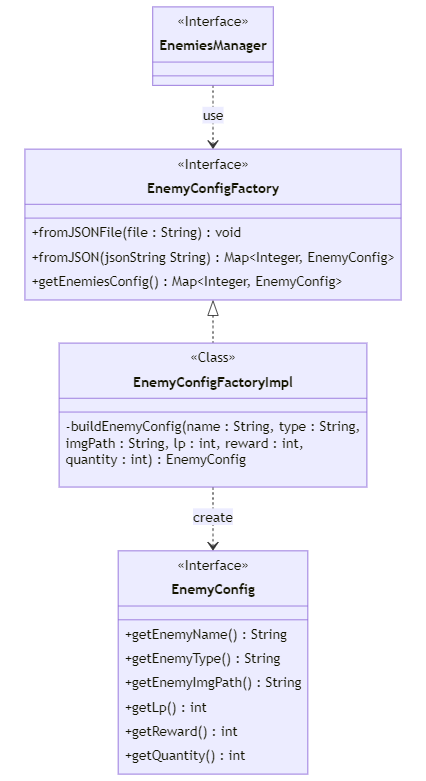
\includegraphics[scale=0.8]{RelazioneTD/images/enemyConfigFactoryUML.png}
    \caption{UML factory per caricamento di configurazioni di nemici}
    \label{fig:enter-label}
\end{figure}

\paragraph{Problema} Il gioco prevede attualmente tre tipologie di nemici, ciascuno con paramentri diversi quali il nome, i punti vita, il reward assegnato con l'uccisione, ecc. che è necessario reperire ogni volta in cui un nemico di quella tipologia viene creato. 
\paragraph{Soluzione} Per garantire futura estendibilità ad ulteriori tipologie di nemici e facile modifica dei parametri è stato deciso di gestire la configurazione dei nemici attraverso un file JSON. Tuttavia, una lettura di questo file in seguito alla creazione di ciascun nemico sarebbe inutilmente dispendiosa del punto di vista delle risorse del sistema. Per questo motivo, si è deciso di sfruttare il pattern factory per creare e salvare in memoria i dati relativi alle varie tipologie di nemici, garantendo un accesso più rapido in fase di generazione degli stessi tramite il metodo \textit{getEnemiesConfig()} dell'interfaccia \textit{EnemyConfigFactory}. In particolare il metodo \textit{fromJSONFile()} è sfruttato da \textit{EnemiesManager} per leggere il file di configurazione e creare attraverso la factory i diversi \textit{EnemyConfig}.

\subsubsection{Gestione dei nemici: spawn, movimento e distruzione}



\newpage
\subsection{Luca Pulga}
\subsubsection{Gestione delle difese}
\paragraph{Problema}
Si vuole gestire in maniera scalabile le varie entità presenti all'interno del gioco, come le difese (torri, armi, proiettili) e i nemici, evitando l'eccessiva scrittura di codice duplicato.

\paragraph{Soluzione}
E' possibile suddividere le varie caratteristiche delle varie entità in sotto-entità, in modo da attribuire le relative proprietà ad ogni tipologia di entità che è presente
o che potrà essere presente in futuro, rendendo la struttura scalabile. Sono state realizzate interfacce e classi astratte, a cui sono state delegate le assegnazioni delle varie proprietà fornendo la condivisione del codice comune e contratti parziali, implementabili dalle sottoclassi.
Un'ulteriore soluzione poteva essere quella di utilizzare solo interfacce e come implementazione di esse, utilizzare i record, in quanto fornirebbero un modo decisamente più coinciso per dichiarare classi immutabili ed eliminerebbero molta della verbosità associata alle classi standard.

\begin{figure}[H]
    \centering
    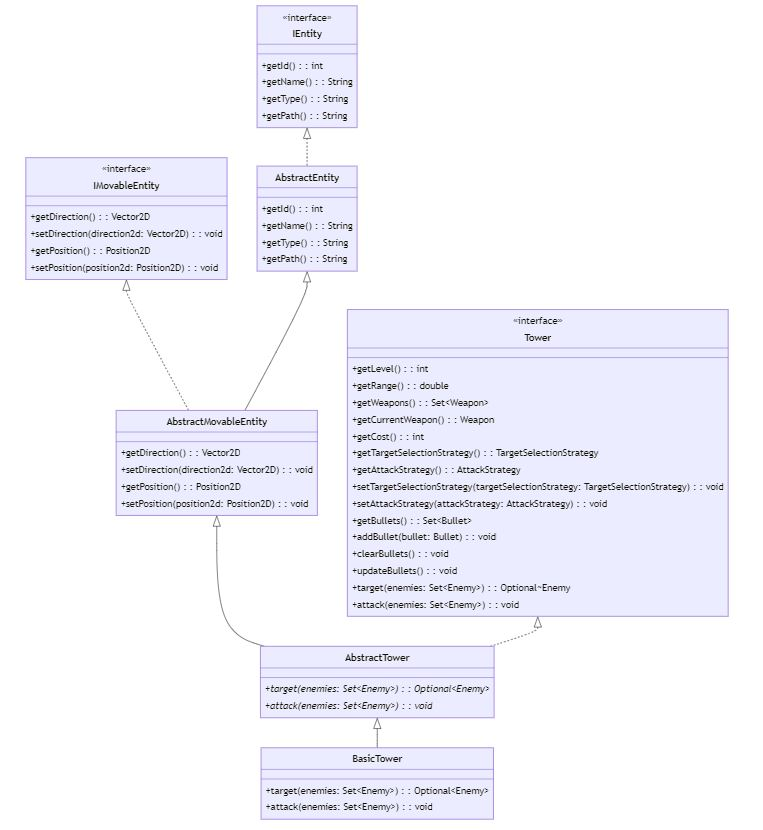
\includegraphics[width=1.2\linewidth]{defense_model.JPG}
    \caption{Figura 2.2: Modello per la gestione delle entità.}
    \label{fig:defense-model}
\end{figure}

\paragraph{Problema}
Disporre di un oggetto in grado di poter creare qualsiasi tipo di entità, centralizzando la parte di creazione degli oggetti che verranno caricati e successivamente utilizzati
durante il gioco.

\paragraph{Soluzione}
Viene utilizzato il \textit{Factory Method Pattern} in modo da sfruttare la sua capacità di separare la costruzione degli oggetti dal loro utilizzo. Dunque questa separazione ci consente di avere una maggiore flessibilità e modularità del codice, rendendolo più facile da mantenere e aggiornare anche introducendo in futuro nuove entità o separare in sotto-entità quelle già esistenti. 
La \textit{Factory} provvederà a leggere i file json all'interno di specifiche cartelle per caricare
le entità, come le \textit{torri}, che saranno poi successivamente gestite dal \textit{Defense Manager}.

\begin{figure}[H]
    \centering
    \includegraphics[width=0.8\linewidth]{entity-factory-method.jpg}
    \caption{Figura 2.3: Factory Method Pattern per il caricamento delle entità.}
    \label{fig:entity-factory-method}
\end{figure}

\paragraph{Problema}
Gestione delle istanze delle torri senza avere un'entità centralizzata.
\paragraph{Soluzione}
La soluzione prevedere l'implementazione di un Defense Manager in grado di gestire le entità difesa. Questa soluzione centralizzata permette di gestire all'interno di un unica classe tutte le entità difesa, fornendo anche un modo comodo all'esterno per ottenere informazioni con altri oggetti.

\begin{figure}[H]
    \centering
    \includegraphics[width=0.8\linewidth]{defense-manager.jpg}
    \caption{Figura 2.4: Defense Manager per la gestione delle difese.}
    \label{fig:defense-manager}
\end{figure}

\paragraph{Problema}:
Implementazione Observer.
\paragraph{Soluzione}:

\begin{figure}[H]
    \centering
    \includegraphics[width=0.8\linewidth]{defense-observer.jpg}
    \caption{Figura 2.5: Defense Manager e Observer.}
    \label{fig:defense-observer}
\end{figure}

\paragraph{Problema}
Implementazione di diverse tipologie di targettamento dei nemici da parte delle torri a seconda della loro tipologia.
\paragraph{Soluzione}
Si implementa il Pattern Strategy, in questo modo il contesto diventa indipendente dalle strategie concrete di targettamento dei nemici, per cui è possibile aggiungere/modificare gli algoritmi di targettamento senza modificare il codice all'interno delle varie classi che potrebbero implementare la relativa strategia di attacco.

\begin{figure}[H]
    \centering
    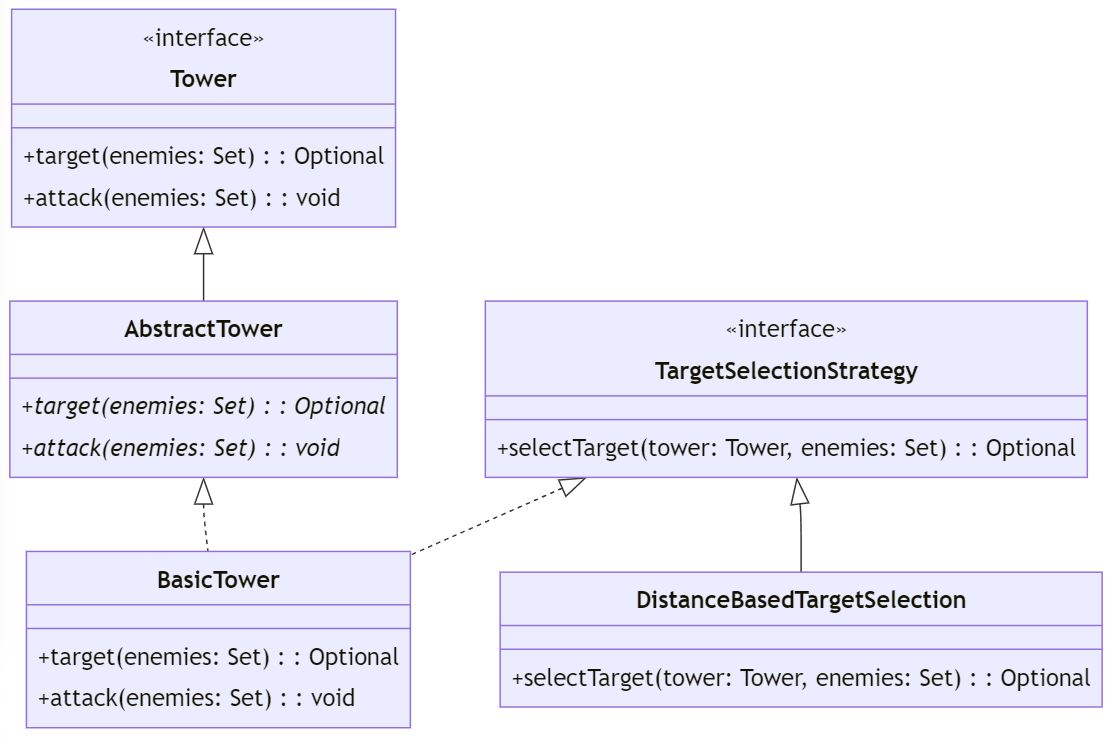
\includegraphics[width=0.8\linewidth]{defense_target.JPG}
    \caption{Figura 2.6: Pattern Strategy per targettamento dei nemici.}
    \label{fig:defense_target}
\end{figure}

\paragraph{Problema}
Implementazione di diverse tipologie di attacchi verso i nemici da parte delle torri a seconda della loro tipologia.
\paragraph{Soluzione}
Si implementa il Pattern Strategy, in questo modo il contesto diventa indipendente dalle strategie concrete di attacco verso i nemici, per cui è possibile aggiungere/modificare gli algoritmi di attacco senza modificare il codice all'interno delle varie classi che potrebbero implementare la relativa strategia di attacco.

\begin{figure}[H]
    \centering
    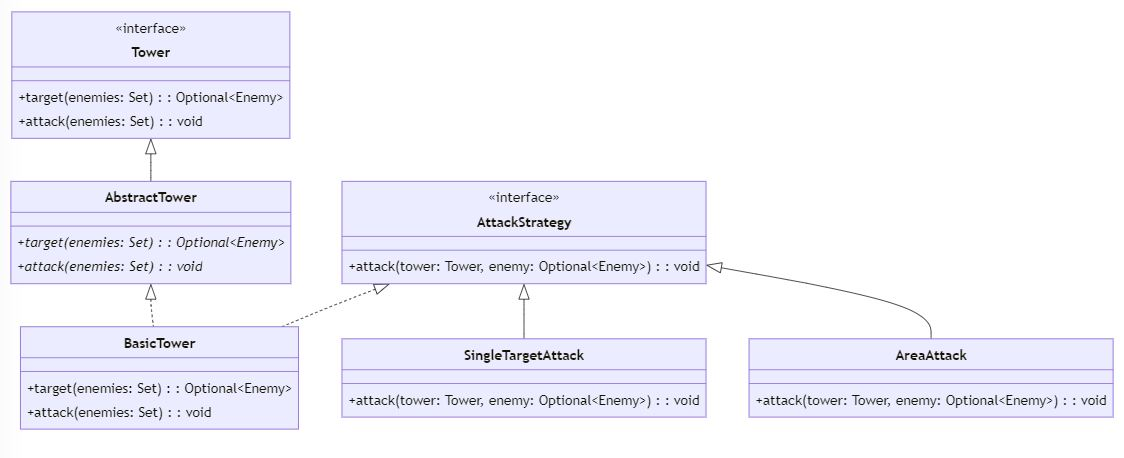
\includegraphics[width=0.8\linewidth]{defense_attack.JPG}
    \caption{Figura 2.7: Pattern Strategy per attacco ai nemici.}
    \label{fig:defense_attack}
\end{figure}

\chapter{Sviluppo}
\section{Testing automatizzato}
Per verificare il corretto funzionamento del gioco Tower-Defense, sono stati creati appositi test automatizzati utilizzando JUnit. 
I test automatizzati sono necessari per poter testare se le logiche pensate durante la fase analisi, di progettazione e di implementazione del Model, e delle classi affini di utility, sono funzionanti.


\begin{itemize}
    \item \textit{\textbf{TestBasicTower}:} Test automatizzato per garantire la correttezza dei metodi di get e set delle difese torri per poter gestire durante il gioco le sue proprietà.
    \item \textit{\textbf{TestBulletImpl}:} Test automatizzato per garantire la correttezza dei metodi di get e set della posizione e direzione del proiettile, fondamentale per la gestione grafica del gioco.
    \item \textit{\textbf{TestDefenseFactory}:} Test automatizzato per garantire la correttezza di lettura da file json delle entità torri attraverso l'utilizzo della \ref{fig:entity-factory-method}EntityFactory
    \item \textit{\textbf{TestTargetStrategy}:} Test automatizzato per garantire la correttezza dei calcoli effettuati durante la fase di targettamento di nemici da parte delle torri.
\end{itemize}

\section{Note di sviluppo}

Questa sezione, come quella riguardante il design dettagliato va svolta \textbf{singolarmente da ogni membro del gruppo}.
%
Nella prima parte, ciascuno dovrà mostrare degli esempi di codice particolarmente ben realizzati,
che dimostrino proefficienza con funzionalità avanzate del linguaggio e capacità di spingersi oltre le librerie mostrate a lezione.

\begin{itemize}
	\item \textbf{Elencare} (fare un semplice elenco per punti, non un testo!) le feature \textit{avanzate} del linguaggio e dell'ecosistema Java che sono state
utilizzate. Le feature di interesse sono:
	\begin{itemize}
		\item Progettazione con generici, ad esempio costruzione di nuovi tipi generici, e uso di generici bounded.
		L'uso di classi generiche di libreria non è considerato avanzato.
		\item Uso di lambda expressions
		\item Uso di \texttt{Stream}, di \texttt{Optional} o di altri costrutti funzionali
		\item Uso di reflection
		\item Definizione ed uso di nuove annotazioni
		\item Uso del Java Platform Module System
		\item Uso di parti della libreria JDK non spiegate a lezione (networking, compressione, parsing XML, eccetera...)
		\item Uso di librerie di terze parti (incluso JavaFX): Google Guava, Apache Commons...
	\end{itemize}
	\item Si faccia molta attenzione a non scrivere banalità, elencando qui features di tipo ``core'', come le eccezioni, le enumerazioni, o le inner class: nessuna di queste è considerata avanzata.
	\item Per ogni feature avanzata, mostrata, includere:
	\begin{itemize}
		\item Nome della feature
		\item Permalink GitHub al punto nel codice in cui è stata utilizzata
	\end{itemize}
\end{itemize}

In questa sezione, \textit{dopo l'elenco},
vanno menzionati ed attributi con precisione eventuali pezzi di codice ``riadattati'' (o scopiazzati...) da Internet o da altri progetti,
pratica che tolleriamo ma che non raccomandiamo.
%
Si rammenta agli studenti che non è consentito partire da progetti esistenti e procedere per modifiche successive.
%
Si ricorda anche che i docenti hanno in mano strumenti antiplagio piuttosto raffinati e che ``capiscono'' il codice e la storia delle modifiche del progetto,
per cui tecniche banali come cambiare nomi (di classi, metodi, campi, parametri, o variabili locali),
aggiungere o togliere commenti,
oppure riordinare i membri di una classe vengono individuate senza problemi.
%
Le regole del progetto spiegano in dettaglio l'approccio dei docenti verso atti gravi come il plagiarismo.

I pattern di design \textbf{non} vanno messi qui.
%
L'uso di pattern di design (come suggerisce il nome) è un aspetto avanzato di design, non di implementazione,
e non va in questa sezione.

\subsection*{Elementi positivi}

\begin{itemize}
	\item Si elencano gli aspetti avanzati di linguaggio che sono stati impiegati
	\item Si elencano le librerie che sono state utilizzate
	\item Per ciascun elemento, si fornisce un permalink
	\item Ogni permalink fa riferimento ad uno snippet di codice scritto dall'autore della sezione (i docenti verificheranno usando \texttt{git blame})
	\item Se si è utilizzato un particolare algoritmo, se ne cita la fonte originale.
	Ad esempio, se si è usato Mersenne Twister per la generazione di numeri pseudo-random, si cita \cite{mersenne}.
	\item Si identificano parti di codice prese da altri progetti, dal web, o comunque scritte in forma originale da altre persone.
	In tal senso, si ricorda che agli ingegneri non è richiesto di re-inventare la ruota continuamente:
	se si cita debitamente la sorgente è tollerato fare uso di di snippet di codice open source per risolvere velocemente problemi non banali.
	Nel caso in cui si usino snippet di codice di qualità discutibile,
	oltre a menzionarne l'autore originale si invitano gli studenti ad adeguare tali parti di codice agli standard e allo stile del progetto.
	Contestualmente, si fa presente che è largamente meglio fare uso di una libreria che copiarsi pezzi di codice:
	qualora vi sia scelta (e tipicamente c'è), si preferisca la prima via.
\end{itemize}

\subsection*{Elementi negativi}
\begin{itemize}
	\item Si elencano feature core del linguaggio invece di quelle segnalate. Esempi di feature core da non menzionare sono:
    \begin{itemize}
        \item eccezioni;
        \item classi innestate;
        \item enumerazioni;
        \item interfacce.
    \end{itemize}
	\item Si elencano applicazioni di terze parti (peggio se per usarle occorre licenza, e lo studente ne è sprovvisto) che non c'entrano nulla con lo sviluppo, ad esempio:
    \begin{itemize}
        \item Editor di grafica vettoriale come Inkscape o Adobe Illustrator;
        \item Editor di grafica scalare come GIMP o Adobe Photoshop;
        \item Editor di audio come Audacity;
        \item Strumenti di design dell'interfaccia grafica come SceneBuilder: il codice è in ogni caso inteso come sviluppato da voi.
    \end{itemize}
	\item Si descrivono aspetti di scarsa rilevanza, o si scende in dettagli inutili.
	\item Sono presenti parti di codice sviluppate originalmente da altri che non vengono debitamente segnalate.
	In tal senso, si ricorda agli studenti che i docenti hanno accesso a tutti i progetti degli anni passati,
	a Stack Overflow,
	ai principali blog di sviluppatori ed esperti Java,
	ai blog dedicati allo sviluppo di soluzioni e applicazioni
	(inclusi blog dedicati ad Android e allo sviluppo di videogame),
	nonché ai vari GitHub, GitLab, e Bitbucket.
	Conseguentemente, è \emph{molto} conveniente \emph{citare} una fonte ed usarla invece di tentare di spacciare per proprio il lavoro di altri.
	\item Si elencano design pattern
\end{itemize}

\subsection{Esempio}

\subsubsection{Utilizzo della libreria SLF4J}

Utilizzata in vari punti.
Un esempio è \url{https://github.com/AlchemistSimulator/Alchemist/blob/5c17f8b76920c78d955d478864ac1f11508ed9ad/alchemist-swingui/src/main/java/it/unibo/alchemist/boundary/swingui/effect/impl/EffectBuilder.java#L49}

\subsubsection{Utilizzo di \texttt{LoadingCache} dalla libreria Google Guava}

Permalink: \url{https://github.com/AlchemistSimulator/Alchemist/blob/d8a1799027d7d685569e15316a32e6394632ce71/alchemist-incarnation-protelis/src/main/java/it/unibo/alchemist/protelis/AlchemistExecutionContext.java#L141-L143}

\subsubsection{Utilizzo di \texttt{Stream} e lambda expressions}

Usate pervasivamente. Il seguente è un singolo esempio.
Permalink: \url{https://github.com/AlchemistSimulator/Alchemist/blob/d8a1799027d7d685569e15316a32e6394632ce71/alchemist-incarnation-protelis/src/main/java/it/unibo/alchemist/model/ProtelisIncarnation.java#L98-L120}

\subsubsection{Scrittura di metodo generico con parametri contravarianti}

Permalink: \url{https://github.com/AlchemistSimulator/Alchemist/blob/d8a1799027d7d685569e15316a32e6394632ce71/alchemist-incarnation-protelis/src/main/java/it/unibo/alchemist/protelis/AlchemistExecutionContext.java#L141-L143}

\subsubsection{Protezione da corse critiche usando \texttt{Semaphore}}

Permalink: \url{https://github.com/AlchemistSimulator/Alchemist/blob/d8a1799027d7d685569e15316a32e6394632ce71/alchemist-incarnation-protelis/src/main/java/it/unibo/alchemist/model/ProtelisIncarnation.java#L388-L440}


\chapter{Commenti finali}
\section{Autovalutazione e lavori futuri}
\subsection{Francesco Aurora}
\subsection{Marco Casali}
\subsection{Cristina Murvai}
\subsection{Luca Pulga}


\textbf{È richiesta una sezione per ciascun membro del gruppo, obbligatoriamente}.
%
Ciascuno dovrà autovalutare il proprio lavoro, elencando i punti di forza e di debolezza in quanto prodotto.
Si dovrà anche cercare di descrivere \emph{in modo quanto più obiettivo possibile} il proprio ruolo all'interno del gruppo.
Si ricorda, a tal proposito, che ciascuno studente è responsabile solo della propria sezione: non è un problema se ci sono opinioni contrastanti, a patto che rispecchino effettivamente l'opinione di chi le scrive.
Nel caso in cui si pensasse di portare avanti il progetto, ad esempio perché effettivamente impiegato, o perché sufficientemente ben riuscito da poter esser usato come dimostrazione di esser capaci progettisti, si descriva brevemente verso che direzione portarlo.


\chapter{Esercitazioni di laboratorio}

\subsection{francesco.aurora@studio.unibo.it}

\subsection{marco.casali13@studio.unibo.it}

\subsection{cristina.murvai@studio.unibo.it}

\subsection{luca.pulga@studio.unibo.it}

\end{document}